%*****************************************
\chapter{Methods}\label{ch:methods}
%*****************************************
%\setcounter{figure}{10}
% \NoCaseChange{Homo Sapiens}
This is just to test whether this template is working
\citeauthor{dueck:trio} \citep{dueck:trio}. His no decore
nemore graecis. In eos meis nominavi, liber soluta vim cu. Sea commune
suavitate interpretaris eu, vix eu libris efficiantur.



\section{Tools and Libraries}
Lorem ipsum quod dolor sit amet.

\subsection{HTK}
Lorem ipsum quod dolor sit amet.

\subsection{Julius}
Lorem ipsum quod dolor sit amet.

\section{Speech Corpora}
Lorem ipsum quod dolor sit amet.

\subsection{TIMIT}
Lorem ipsum quod dolor sit amet.

\subsection{WSJ0}
Lorem ipsum quod dolor sit amet.

\subsection{SpeechDat}
Lorem ipsum quod dolor sit amet.

\subsection{Listener's Corpus}
Lorem ipsum quod dolor sit amet.

\section{Building the Acoustic Model}

\subsection{The Phoneset}\label{sec:listener-phoneset}

Since our goal is to build an \ac{ASR} system capable of recognizing non-native speech, we propose
to use an interlingual phoneset as the basis of the pronunciation model. By doing this, we can define
\ac{HMM} models for estimating phones which are part of both the speaker's native language (\ac{BP}) and 
target language (\ac{AmE}).

A straightforward approach would be to look up the literature in phonetics and phonology in order to find
a \ac{BP}--\ac{AmE} interlingual phoneset. However, to the best of our knowledge, no researches were carried 
out in this regard. There are papers addressing specific mispronunciations, such as (XXXX INSERT CITATIONS) , 
which list some occurring interlingual phones, but there is not a wide-ranging study available about this matter.

Therein we had to develop our own interlingual phoneset. For simplicity, we decided to use the union set formed 
by the phones in two machine-readable dictionaries, one for \ac{AmE}: \ac{CMUdict} \cite{CMU2008}, and another for \ac{BP}: 
Aeiouad\^o \cite{Mendonca2014}. By doing this, we can cover most of the phone productions brazilian ESL students are likely
to make. Advanced students will tend to use more proper \ac{AmE} phones, whereas beginners will have a stronger accent,
thus using more phones from the \ac{BP} dictionary. A brief description of each of these dictionaries is given below, before 
we go into further details of our interlingual set.


\ac{CMUdict} \citep{CMU2008} is a machine-readable pronunciation dictionary for \ac{AmE} which contains about $125,000$ 
words and their transcriptions. It was designed primarily for speech applications, such as speech recognition and synthesis, 
and it has been widely tested in both Academia and industry (XXX INSERT CITATIONS).

Words in \ac{CMUdict} are transcribed using ARPAbet, a phonetic transcription code developed by the Advanced Research Projects Agency in 
$1971$. It represents each \ac{AmE} phone with a distinct sequence of \ac{ASCII} characters. In the dictionary, there are in total $39$ 
phones plus stress marks. The phone convention is described on \autoref{tab:cmu-conv}.

\begin{table}[p]
  \caption[CMUdict phone convention.]{CMUdict phone convention.}
  \smallskip
  \centering
  \begin{tabular}{ccccc} \toprule
      \tableheadline{\#} & \tableheadline{CMU Phone} & \tableheadline{IPA Phone} & \tableheadline{Example} & \tableheadline{Transcription} \\ \midrule
      1 & AA & [\textipa{A}] & odd & AA D \\
      2 & AE & [\textipa{ae}] & at & AE T \\
      3 & AH & [\textipa{@}] & hut & HH AH T \\
      4 & AO & [\textipa{O}] & ought & AO T \\
      5 & AW & [\textipa{aU}] & cow & K AW \\
      6 & AY & [\textipa{aI}] & hide & HH AY D \\
      7 & B & [\textipa{b}] & be & B IY \\
      8 & CH & [\textipa{tS}] & cheese & CH IY Z \\
      9 & D & [\textipa{d}] & dee & D IY \\
      10 & DH & [\textipa{D}] & thee & DH IY \\
      11 & EH & [\textipa{E}] & Ed & EH D \\
      12 & ER & [\textipa{@r}] & hurt & HH ER T \\
      13 & EY & [\textipa{A\*r}] & ate & EY T \\
      14 & F & [\textipa{f}] & fee & F IY \\
      15 & G & [\textipa{g}] & green & G R IY N \\
      16 & HH & [\textipa{h}] & he & HH IY \\
      17 & IH & [\textipa{I}] & it & IH T \\
      18 & IY & [\textipa{i}] & eat & IY T \\
      19 & JH & [\textipa{dZ}] & gee & JH IY \\
      20 & K & [\textipa{k}] & key & K IY \\
      21 & L & [\textipa{l}] & lee & L IY \\
      22 & M & [\textipa{m}] & me & M IY \\
      23 & N & [\textipa{n}] & knee & N IY \\
      24 & NG & [\textipa{N}] & ping & P IH NG \\
      25 & OW & [\textipa{oU}] & oat & OW T \\
      26 & OY & [\textipa{OI}] & toy & T OY \\
      27 & P & [\textipa{p}] & pee & P IY \\
      28 & R & [\textipa{\*r}] & read & R IY D \\
      29 & S & [\textipa{s}] & sea & S IY \\
      30 & SH & [\textipa{S}] & she & SH IY \\
      31 & T & [\textipa{t}] & tea & T IY \\
      32 & TH & [\textipa{T}] & theta & TH EY T AH \\
      33 & UH & [\textipa{U}] & hood & HH UH D \\
      34 & UW & [\textipa{u}] & two & T UW \\
      35 & V & [\textipa{v}] & vee & V IY \\
      36 & W & [\textipa{w}] & we & W IY \\
      37 & Y & [\textipa{y}] & yield & Y IY L D \\
      38 & Z & [\textipa{z}] & zee & Z IY \\
      39 & ZH & [\textipa{Z}] & seizure & S IY ZH ER \\
    \bottomrule
  \end{tabular}
  \label{tab:cmu-conv}
\end{table}

Aeiouad\^o\footnote{Aeiouad\^o is byproduct of this dissertation, it was developed within my Master's Course. 
It is available at: \url{http://nilc.icmc.usp.br/listener/aeiouado}} \citep{Mendonca2014}
is a machine-readable pronunciation dictionary for \ac{BP}. Its transcriptions are based on the dialect of S\~ao Paulo city
and contains 39 different phones. The dictionary makes use of a hybrid approach for converting graphemes into phonemes, 
which employs both manual transcription rules and machine learning algorithms. It was compiled from an available dump of the 
Portuguese Wikipedia, on January $23$\textsuperscript{rd} $2014$. 

The articles  were transformed into plain text, tokenized and word types were extracted. A language identification tool was developed 
to detect loanwords among data. Words' syllable boundaries and stress were identified. The transcription task was carried
out in a two-step process: i) words were submitted to a set of transcription rules; ii) a machine learning classifier was 
used to predict the transcription of the remaining graphemes. The method was evaluated through $5$-fold cross-validation; 
and results showed a high F$1$-score: $0.98$.

\begin{table}[p]
  \caption[Aeiouad\^o phone convention.]{Aeiouad\^o phone convention.}
  \smallskip
  \centering
  \begin{tabular}{ccccc} \toprule
      \tableheadline{\#} & \tableheadline{Aeiouad\^o Phone} & \tableheadline{IPA Phone} & \tableheadline{Example} & \tableheadline{Transcription} \\ \midrule
      1 & a & [\textipa{a}] & amor & a m o x \\
      2 & a$\sim$ & [\textipa{\~a}] & canto & k a$\sim$ t U \\
      3 & b & [\textipa{b}] & besta & b e s t @ \\
      4 & d & [\textipa{d}] & da & d a \\
      5 & dZ & [\textipa{dZ}] & dia & dZ i @ \\
      6 & E & [\textipa{E}] & \'e & E \\
      7 & e & [\textipa{e}] & dedo & d e d U \\
      8 & e$\sim$ & [\textipa{\~e}] & venda & v e$\sim$ d @ \\
      9 & f & [\textipa{f}] & frio & f 4 i U \\
      10 & g & [\textipa{g}] & gula & g u l @  \\
      11 & G & [\textipa{G}] & carga & carga \\
      12 & i & [\textipa{i}] & a\'i & a i \\
      13 & I & [\textipa{I}] & come & k o$\sim$ m I \\
      14 & i$\sim$ & [\textipa{\~i}] & sim & s i$\sim$ \\
      15 & J & [\textipa{\textltailn}] & ganho & g a$\sim$ J U \\
      16 & j & [\textipa{y}] & pai & p a j \\
      17 & j$\sim$ & [\textipa{\~y}] & parem & p a 4 e$\sim$ j$\sim$ \\
      18 & k & [\textipa{k}] & compra & k o$\sim$ p 4 @ \\
      19 & l & [\textipa{l}] & l\'a & l a \\
      20 & L & [\textipa{L}] & palha & p a L @ \\
      21 & m & [\textipa{m}] & m\~ae & m a$\sim$ j$\sim$ \\
      22 & n & [\textipa{n}] & n\~ao & n a$\sim$ w$\sim$ \\
      23 & O & [\textipa{O}] & p\'o & p O \\
      24 & o & [\textipa{o}] & gorro & g o x U \\
      25 & o$\sim$ & [\textipa{\~o}] & com & k o$\sim$ \\
      26 & p & [\textipa{p}] & pessoa & p e s o @ \\
      27 & s & [\textipa{s}] & susto & s u s t U \\
      28 & t & [\textipa{t}] & tato & t a t U \\
      29 & tS & [\textipa{tS}] & noite & n o j tS I \\
      30 & u & [\textipa{u}] & durmo & d u G m U \\
      31 & U & [\textipa{U}] & c\'umulo & k u m u l U \\
      32 & u$\sim$ & [\textipa{\~u}] & um & u$\sim$ \\
      33 & v & [\textipa{v}] & vida & v i d @ \\
      34 & w & [\textipa{w}] & aula & a w l @ \\
      35 & w$\sim$ & [\textipa{\~w}] & canh\~ao & k a$\sim$ J a$\sim$ w$\sim$ \\
      36 & x & [\textipa{x}] & rato & x a t U \\
      37 & z & [\textipa{z}] & zebra & z e b 4 @ \\
      38 & 4 & [\textipa{R}] & arara & a 4 a 4 @ \\
      39 & @ & [\textipa{@}] & bola & b O l @ \\
    \bottomrule
  \end{tabular}
  \label{tab:aeiouado-conv}
\end{table}

In what concerns to our interlingual phoneset, an analysis from both dictionaries shown that many \ac{BP} and \ac{AmE} phones overlap,
as expected. This is true specially for consonants, [\textipa{b}, \textipa{d}, \textipa{dZ}, \textipa{f}, \textipa{g}, \textipa{k}, 
\textipa{l}, \textipa{m}, \textipa{n}, \textipa{p}, \textipa{s}, \textipa{t}, \textipa{tS}, \textipa{v}, \textipa{z}] appear on both 
languages. Several vowels also do overlap, [\textipa{E}, \textipa{i}, \textipa{I}, \textipa{O}, \textipa{u}, \textipa{U}, \textipa{@}],
together with both glides [\textipa{y}, \textipa{w}].

However it is worth noticing that of some these segments are not exactly the same. The production of [\textipa{p},\textipa{t},\textipa{k}], 
for instance, in \ac{BP} and \ac{AmE} can be quite different. In English, it is known that when such consonants 
occur in certain contexts, for example, in word initial position or onset of a stressed syllable, they become aspirated; whence
[\textipa{p\super h},\textipa{t\super h},\textipa{k\super h}] \citep{Lisker1985}. 
This process is not found in \ac{BP}, where, disregard of the context, [\textipa{p},\textipa{t},\textipa{k}] show no 
relevant values of aspiration \citep{Klein1999}. For that reason, in order to properly estimate \ac{HMM} states, it is 
better in this case to create aspirated phone models for these consonants, and then map the aspirated realizations onto them.

For that reason, we analysed each of the cases 


\subsection{HMM topology}

\subsection{Tree-Based State Tying}

Data-driven approaches also show limitations. Since such approaches are generally based on 
the positive examples which occur in a corpus, rare or non-occuring phenomena are often poorly estimated or even neglected.
This is the case for triphone \ac{HMM} models. 

Natural languages have, on average, $30$ different phones. The language believed to have the smallest phonetic inventory is 
Rotokas (East Papuan, New Guinea), with 11 phones, and the one with largest is !X\'o\~o  (Khoisan, Botswana/Namibia), 
with 160 \citep{Hayes2011}. English is usually assumed to have 37 to 41 phones, depending on the dialect. 

In the \ac{CMUdict} \citep{CMU2008}, 39 phones are used to describe the words of \ac{AmE}. When it comes to triphones, in theory, 
this number might grow by three orders of magnitude, that is $39^3$ or $59,319$. It is true that due to phonotactic constraints
many of the virtually possible triphones never take place in practice. 
For instance, the triphone sequence [\textipa{N}-\textipa{s}+\textipa{p}] does not exist in English, although it 
is made of valid and existing monophones [\textipa{N}], [\textipa{s}] and [\textipa{p}]. 

\citeauthor{Kuperman2008} \citep{Kuperman2008} examined the monophone, diphone and triphone frequencies in speech corpora
for many languages. In what concerns to English, they analysed the Buckeye Corpus and reported that it contains $29,804$ different 
occurring triphones (or types), distributed among $431,000$ tokens. Although the actual number of triphones for English is
almost half the number of possible permutations, it is still a huge number of triphones to model over a corpus. 
Therefore, in order to build an \ac{ASR} system, one always has to deal with data scarcity and try to overcome its limitations.

Within \ac{HMM} \ac{ASR}, tree-based state tying is a technique to improve the modelling of rare triphones and allow the 
estimation of non-occurring ones. It was initially proposed by \citeauthor{Young1994} \citep{Young1994} and since then
has become a standard procedure in \ac{HMM} \ac{ASR} systems. The aim of tree-based state tying is to maintain the balance 
between the model complexity and the available training data by tying the \ac{HMM} states of acoustically similar triphones.

In contrast to the majority of methods in \ac{ASR}, tree-based state tying is carried out in a top-down, knowledge-based 
way. A specialist (generally a speech sciencist, phologist or phoneticist) uses his/her knowledge to build a phonetic decision 
tree which will organize the phones into sets with similar acoustic parameters. 

In most cases, the criteria used to organize phones into a decision tree are the so-called natural classes. 
Natural classes were proposed within the generative phonology framework. In this framework, phones and and phonemes are no 
longer considered the basic units of analysis, instead it is assumed that they can be broken down into smaller components,
which describe aspects of articulation and perception, such as [+nasal], [-continuant], [+strident], etc. For instance,
the phone [\textipa{s}] would not be represented in generative phonology as a single phonetic symbol [\textipa{s}], but 
as a bundle of distinctive features \citep{Jensen2004}:
\[
[{\textipa{a}}] \rightarrow 
\begin{bmatrix}
+consonantal \\ -syllabic \\ -sonorant \\ +continuant \\ +anterior \\ +coronal \\ +strident \\ -voiced
\end{bmatrix}
\]

Distinctive features were probably the most important contribution of generative phonology. They became popular as a
model specially because they were able of simplify phonological processes by grouping segments. Consider the case of
final-obstruent devoicing. In many pronunciations of Standard German, voiced obstruent consonants become devoiced when
they occur in word final position. This is the case for a large number of german nouns which make their plural by the 
addition of the suffix \{-\textipa{e}\}. \autoref{tab:german-devoicing} contains a few examples extracted from 
\citeauthor{} \citep{}.

\begin{table}[!htb]
  \caption[Examples of final-obstruent devoicing in German.]{Examples of final-obstruent devoicing in German.}
  \smallskip
  \centering
  \begin{tabular}{ccc} \toprule
    \tableheadline{Plural form} & \tableheadline{Singular form} & \tableheadline{Gloss} \\ \midrule
    Die[\textipa{b}]e & Die[\textipa{p}] & \small{thief} \\
    Hun[\textipa{d}]e & Hun[\textipa{t}] & \small{dog} \\
    Ber[\textipa{g}]e & Ber[\textipa{k}] & \small{mountain} \\
    M\"au[\textipa{z}] & Mau[\textipa{s}] & \small{mouse} \\
    \bottomrule
  \end{tabular}
  \label{tab:german-devoicing}
\end{table}

As one can observe at the provided examples, the plural forms contain only voiced obstruents whilst the singular forms contain their 
devoiced counterparts. To express this phonological process within structural phonology, one would have to introduce at
least four rules:
\[
[\textipa{b}] \rightarrow [\textipa{p}]  / \_ \# 
\]
\[
[\textipa{d}] \rightarrow [\textipa{t}]  / \_ \#
\]
\[
[\textipa{g}] \rightarrow [\textipa{k}]  / \_ \#
\]
\[
[\textipa{d}] \rightarrow [\textipa{s}]  / \_ \#
\]

Whereas using distinctive features, all cases of german final-obstruent devoicing can be explained by a single rule:
\[
\begin{bmatrix}
+consonantal \\ -syllabic \\ -sonorant \\ +voiced
\end{bmatrix} \rightarrow 
\begin{bmatrix}
-voiced
\end{bmatrix}
 / \_ \#
\]

The main benefits of distinctive features lie in their capability of making generalizations, that is to say
of grouping phones together in a meningful way.  Phonologists have long known that sounds that share the same manner, 
place of articulation, or voicing level behave similarly. Distinctive features provide a way to express this
in an elegant way, by stablishing that feature matrices which are not fully specified do form a natural class. 
Therefore a distinctive features matrix
\[
\begin{bmatrix}
+consonantal \\ -syllabic
\end{bmatrix}
\]
represents all consonants,
\[
\begin{bmatrix}
+consonantal \\ -syllabic \\ +continuant \\ +voiced
\end{bmatrix}
\]
represents all voiced fricatives, etc. For developing the phonetic decision tree, the specialist employs his/her 
knowledge of phonetics and phonology in order to define questions about the phonetic environment of a given 
phone. This phonetic environment is defined by using natural classes, such that an example question would
be ``is the phone preceded by an obstruent?'' or ``is there fricative after the phone?'' Technically, the tree is a 
binary one, i.e a connected acyclic graph such that the degree of each vertex is no more than three. Each
internal node of the tree represents a question about the phonetic context a triphone, each branch represents the answer in a yes-no
form and leaf nodes define \ac{HMM} states. Once the tree is built, its structure is used to decide how \ac{HMM} states will
be tied among triphone models. \autoref{fig:decision-tree} presents an example of a phonetic decision tree.

\begin{figure}[!htb]
        \myfloatalign
        {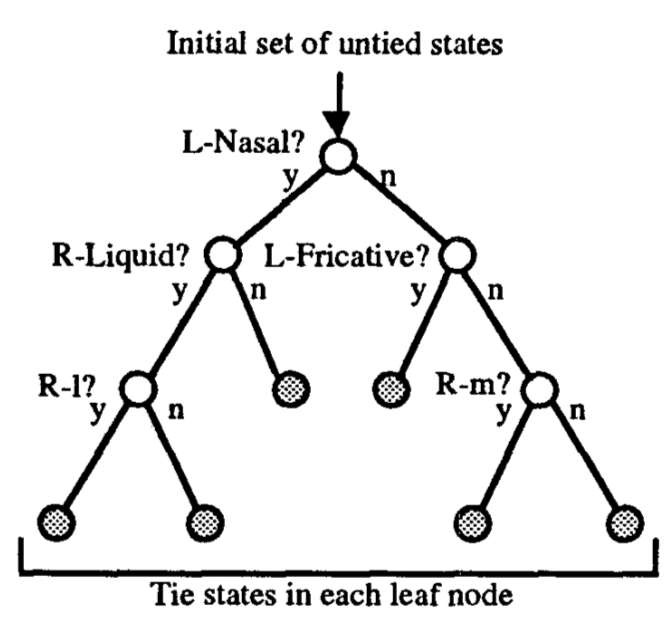
\includegraphics[width=.66\linewidth]{gfx/decision-tree.png}}
        \caption{Phonetic decision tree for HMM state tying \citep{Young1994}.}
        \label{fig:decision-tree}
\end{figure}

The tree input is each triphone being analysed. The first node (the root of the tree) checks if the left 
part of the triphone contains a nasal consonant. If positive, the tree examines the right side of the triphone, by questioning
whether it is a liquid consonant. If negative, a leaf is reached and the HMM state to be tied is outputted, e.g. ``tie
the 1\textsuperscript{st} emitting HMM state of the analysed triphone $A$ to [Nasal-A+*]''.

Formally a phonetic decision tree can be defined as a graph G(e,v) .... (XXXXX INSERT HERE FORMAL DEFINITION)

\autoref{fig:state-tying-tree} summarizes the state tying procedure.

\begin{figure}[!htb]
        \myfloatalign
        {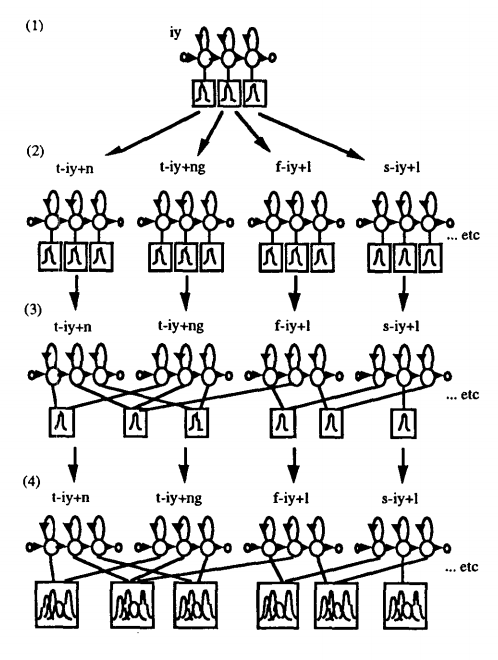
\includegraphics[width=.66\linewidth]{gfx/state-tying-tree.png}}
        \caption{Tied-state HMM system build procedure \citep{Young1994}.}
        \label{fig:state-tying-tree}
\end{figure}

For building the phonetic decision tree for Listener, we based ourselves on the distinctive feature set proposed by 
\citeauthor{Jensen2004} \citep{Jensen2004}, which follows the main guidelines of generative phonology by dividing
the features into four central classes: i) major class features, ii) manner features; iii) place features; and 
iv) laryngeal features.

In practice, classes work as following. Major class features distinguish among the most general classes of sound, 
i.e. vowels, consonants and glides (or semi-vowels). Manner features determine how sounds are articulated, 
that is do they consist of a stop, a nasal, a fricative, a liquid, a trill or a flap? Place features describe 
where in the mouth sounds are produced, whether in the labial region, the alveolar region, the velar region, etc.
Finally, laryngeal features represent the glottal states of sounds, their basic purpose is to differ voiced 
sounds from unvoiced ones.

\citeauthor{Jensen2004} \citep{Jensen2004} proposes a set of $17$ features to describe most of the world languages.

\begin{enumerate}
 \item \emph{Major class features}: syllabic, consonantal and sonorant;
 \item \emph{Manner features}: continuant, nasal, lateral, strident and delayed release;
 \item \emph{Place features}: anterior, coronal, distributed, high, low, back, advanced tongue root (abbreviated as \ac{ATR}) and round.
 \item \emph{Laryngeal features}: voice and heightened subglottal pressure (abbreviated as \ac{HSP});
\end{enumerate}

The somewhat reduced set for place features is capable of representing a large amount of places of articulation 
since features which are regularly restricted to vowels (such as high, low, back and round) are also shared 
with consonants. Besides, once features have a binary nature, therefore, in theory, a number $n$ of features is able
to dintinguish up to $2^n$ phones. In \autoref{fig:features-place}, a comparison is shown between place features and their corresponding
regions of articulation. For a full explanation of each feature, please see \citeauthor{Jensen2004} \citep{Jensen2004}.

\begin{figure}[!htb]
        \myfloatalign
        {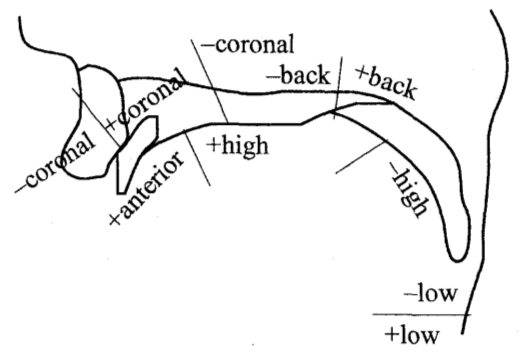
\includegraphics[width=.66\linewidth]{gfx/features-place.png}}
        \caption{Distinctive features for places of places of articulation \citep{Jensen2004}.}
        \label{fig:features-place}
\end{figure}

According to this set of distinctive features, we can arrange the entire phonetic inventory of \ac{AmE} as in \autoref{}.

Afterwards, 


\section{Building the Pronunciation Model}

To the best of our knowledge, no previous research has addressed the problem of generating brazilian-accented 
transcriptions for an \ac{ASR} purposes. Therefore we had to develop our own pronunciation model
\footnote{``Pronunciation models'' are also called ``pronunciation dictionaries''. In this dissertation, we are going to use both terms interchargeably, without distinction.}
. There are basically 
three main approaches we could use to build such model: rule-based methods (XXX CITATION), machine learning methods (XXX CITATION)
and hybrid ones (XXX CITATION). For achieving good performance through machine learning or hybrid approaches, one necessary 
needs a large annotated corpus. That is not the case though. The only Brazilian-accented transcribed corpus we have access
is the Listener Corpus, but we carried out some pilot experiments that showed it was not robust enough for the task.

That being so, we decided to make use of a rule-based approeach for building the pronunciation model. We reviewed all papers 
described in \autoref{ch:second-language}, that deal with the mispronunciation of \ac{AmE} phones by brazilians, in order to find 
interlingual allophonies, such as the English [\textipa{T}] usually becomes [\textipa{t}], [\textipa{t\super h}] or [\textipa{f}] in 
beginners' speech \citep{Reis2006}. 

By knowing the allophonies, we developed rules in order to generate the mispronunciations in the dictionary. It is worth mentioning that,
for creating the rules, we took into account the frequency of occurrence of each mispronunciation (when this information was available 
on the papers). Therefore, mispronunciations which were reported as being very rare or with no significant probability were excluded.
The pseudocode for each mispronunciation pattern is described below. The following conventions apply to all pseudocode examples:

\begin{enumerate}
 \item phonetic transcriptions are placed between brackets and follow the Listener phoneset convention ]
 (see \autoref{sec:listener-phoneset}), therefore [\textipa{"hElow}] becomes [hh eh l ow];
 \item ortographic forms are placed between angle brackets, like <hello>;
 \item the dollar sign ``\$'' represents word final boundary, whether in phonetic or ortographic transcription, thus [ih d\$] means that the transcription ends in [ih d];
 \item the caret symbol ``\textasciicircum'' denotes word initial boundary, whether in phonetic or ortographic transcription, thus <\textasciicircum st> means that word begins with <\textasciicircum st>.
\end{enumerate}

\subsection{Syllable Simplification}
Rules for syllable simplification were created upon production data reported on the following works:
\citeauthor{Cardoso2011} \citep{Cardoso2011}, \citeauthor{Silveira2012} \citep{Silveira2012}
\citeauthor{Rauber2004} \citep{Rauber2004}, and \citeauthor{Rebello2007} \citep{Rebello2007}. The rules
encompass three major cases of syllable simplification. The first one refers to stop consonants in word 
final position, such as the final [\textipa{p}] in ``pop'' which is likely to be produced by learners
together with an epenthetic vowel [\textipa{I}], whence [\textipa{"p\super hApI}]. The second case regards written language
influencing the learner's pronunciation. 

ii) Written language influencing pronunciation
iii) Initial /sC/ clusters 

\lstinputlisting[caption=Pronunciation rules for generating syllable simplification mispronunciations]%
    {Examples/pseudo-rules-syll-simplif.txt}

\subsection{Consonant Change}
\subsection{Deaspiration of Voiceless Plosives in Initial or Stressed Positions}
\subsection{Terminal Devoicing in Word-Final Obstruents}
\subsection{Delateralization and rounding of lateral liquids in final position}
\subsection{Vocalization of final nasals}
\subsection{Velar consonantal paragoge}
\subsection{Vowel assimilation}
\subsection{Interconsonantal epenthesis (-ed and -s morphemes)}






%*****************************************
%*****************************************
%*****************************************
%*****************************************
%*****************************************
